\chapter{Обзор Литературы} \label{chapt1}
% ОПРЕДЕЛЕНИЕ РАДИАЦИОННОЙ НАГРУЗКИ В КОСМИЧЕСКОМ АППАРАТЕ ПРИ ПОЛЕТЕ ПО ВЫСОКОШИРОТНОЙ ОРБИТЕ

\section{Радиационная обстановка на высокоширотных околоземных орбитах. } \label{sect1_1}

Исследования радиационной обстановки в космическом пространстве связано с началом полетов автоматических аппаратов и человека в космос.  Широкое распространение технологий, связанных с использованием космической техники, а также непрерывные пребывание человека в космическом пространстве во время миссий на космических станциях МИР и МКС позволило выявить ряд опасностей космических полетов, среди которых особое внимание следует уделить радиационной опасности \cite{logachev2007}.


Запуск 2-го и 3-го спутников Земли, с приборами, изготовленными в НИИЯФ~МГУ,  
показал принципиальную возможность полета человека в космос.  Еще из данных полученных при первых исследованиях радиационной 
обстановки был сделан вывод, что на орбите земли существуют отдельные области повышения радиационного фона (Рисунок \ref{fig:cylindricalpoes200310mep}). Существование данных областей связано с неоднородностями 
магнитного поля Земли и приводит к формированию области повышения потоков 
частиц в 
Южно Атлантической области \cite{logachev2007}, названной Южно-Атлантической 
Аномалией (ЮАА), как показано в статье Вернова С.Н.\cite{vernov1961}. В первом 
приближении для описания магнитного поля  Земли на высотах до 2000 км можно 
использовать представление модели смещенного диполя, этот подход позволяет 
учитывать ЮАА.

\begin{figure}
	\centering
	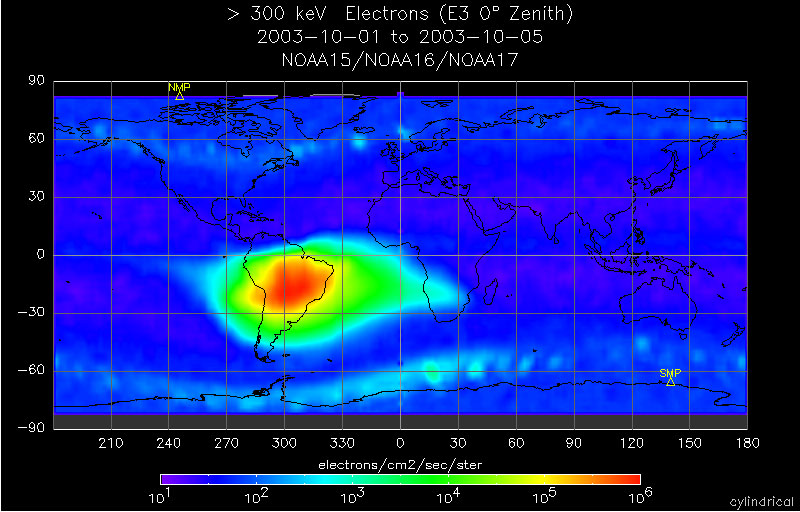
\includegraphics[width=0.7\linewidth]{images/cylindrical_poes_200310_mep}
	\caption{Измерения потоков электронов >300 кэВ на спутнике POES \cite{Peck2008}}
	\label{fig:cylindricalpoes200310mep}
\end{figure}

%Сошлёмся на библиографию. Одна ссылка: \cite[с.~54]{Sokolov}\cite[с.~36]{Gaidaenko}. Две ссылки: \cite{Sokolov,Gaidaenko}. Много ссылок:  \cite[с.~54]{Lermontov,Management,Borozda}


Рисунок Распределение потоков частиц по данным 2-го корабля-спутника над поверхностью земного шара на высоте 320 км. (цифpы у линий дают потоки частиц в см\textsuperscript{-2} c\textsuperscript{-1}) \cite{logachev2007}.


Таким образом, магнитное поле Земли экранирует космические аппараты, находящиеся на средних широтах и невысоких орбитах порядка трехсот-четырехсот километров от поверхности Земли (именно на этих высотах поддерживается обращение космических станций). Значительный вклад, до 60\%,  в дозовую нагрузку аппараты и их экипаж получают в ЮАА, поэтому важную роль  при прогнозировании дозы является точное определение дозы в ЮАА\cite{lish2014, Lishnevskii2012}.

\begin{figure}
	\centering
	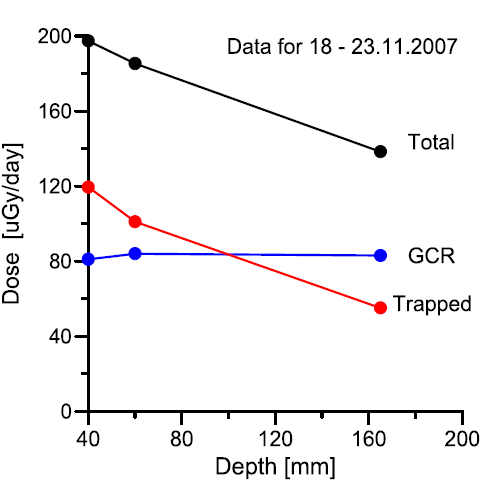
\includegraphics[width=0.7\linewidth]{images/liulinGCRSAA}
	\caption{Вклад в общую поглощенную дозу от ГКЛ и ЮАА. По материалам  \cite{Dachev2015}}
	\label{fig:liulingcrsaa}
\end{figure}

Особенно важными с точки зрения радиационной обстановки, являются приполярные области \cite{gorchakov1961}. При выборе более высокоширотных и высоких орбит они требуют дополнительного внимания, так как в этих областях границы радиационных поясов Земли ближе к поверхности. Даже на небольших высотах, начиная от 300 км в интервале геомагнитных широт 55-70 наблюдается резкое возрастание интенсивности излечения и частицами, составляющими этот внешний радиационный пояс являются электроны различных энергий, их поток достигает 10\textsuperscript{5} см\textsuperscript{-2} сек\textsuperscript{-1} стер\textsuperscript{-1} \cite{vernov1960}. При солнечных событиях в этих областях создаются условия для многократного повышения потоков частиц, что может привести к необходимости специальных мер по предотвращению чрезмерной радиационной нагрузке на экипаж космического аппарата.

\subsection{Вопросы, требующие детального исследования}
Происхождение и динамика потоков релятивистских электронов во внешнем радиационном поясе до сих пор вызывает активный интерес мирового сообщества, несмотря на множество исследований  за более чем пол века исследований \cite{Gussenhoven1997,Borovsky2010,Holeman1991,Miyoshi2011,Chen2016,Turner2013,Brautigam2001,Borovsky2010a,Gussenhoven1995,Borovsky2011,Baker2013,Mullen1998,Chen2014,Morley2010,Potapov2014,Denton2010}. Этот интерес определяется в первую очередь радиационной опасностью, которую представляют экстремально высокие потоки электронов для аппаратов на орбитах полярных спутников. Серьезность радиационных рисков, связанных с энергичными электронами подтверждается в проектах по построению искусственных орбитальных конструкций предназначенных для снижения заселенности внешнего электронного пояса с помощью электростатических полей \cite{Hoyt2007}.

Современные исследования показывают возможность проникновения электронов высоких энергий и в область внутренноего пояса \cite{Claudepierre2017}. Такие выводы были сделаны на основе анализа данных по потокам электронов со спутников Themis во время магнитных бурь. Благодаря нескольким приборам MagEIS  на каждом КА Themis и магнитному разделению частиц по энергиям, стало возможно получать не только потоки частиц но и питч-угловое распределение. Подробный анализ динамики радиационных поясов за 2015 год показал что электроны в зазоре между поясами могут существовать до десятков дней, а во внутреннем поясе до полутора лет \cite{Claudepierre2017}. 

Темне менее существует мнение что обнаружение релятивистских  электронов во внутреннем поясе на самом деле может быть аппаратурной неоднозначностью - совпадением при одновременной регистрации  протонов внутреннего пояса и низкоэнергичных электронов \cite{Selesnick2015}. Численное моделирование спектрометров заряженных частиц также показывает что надежное разделение протонов и электронов возможно только при очень строгих критериях отбора заложенных в логику работы приборов \cite{zolotarev2017numerical51590279}. Сужение критериев  приводит к огромному падению чувствительности прибора и действующего геометрического фактора, для некоторых энергетических каналов возможно снижение до 100 раз \cite{zolotarev2017numerical51590279}.
 
\begin{figure}
	\centering
	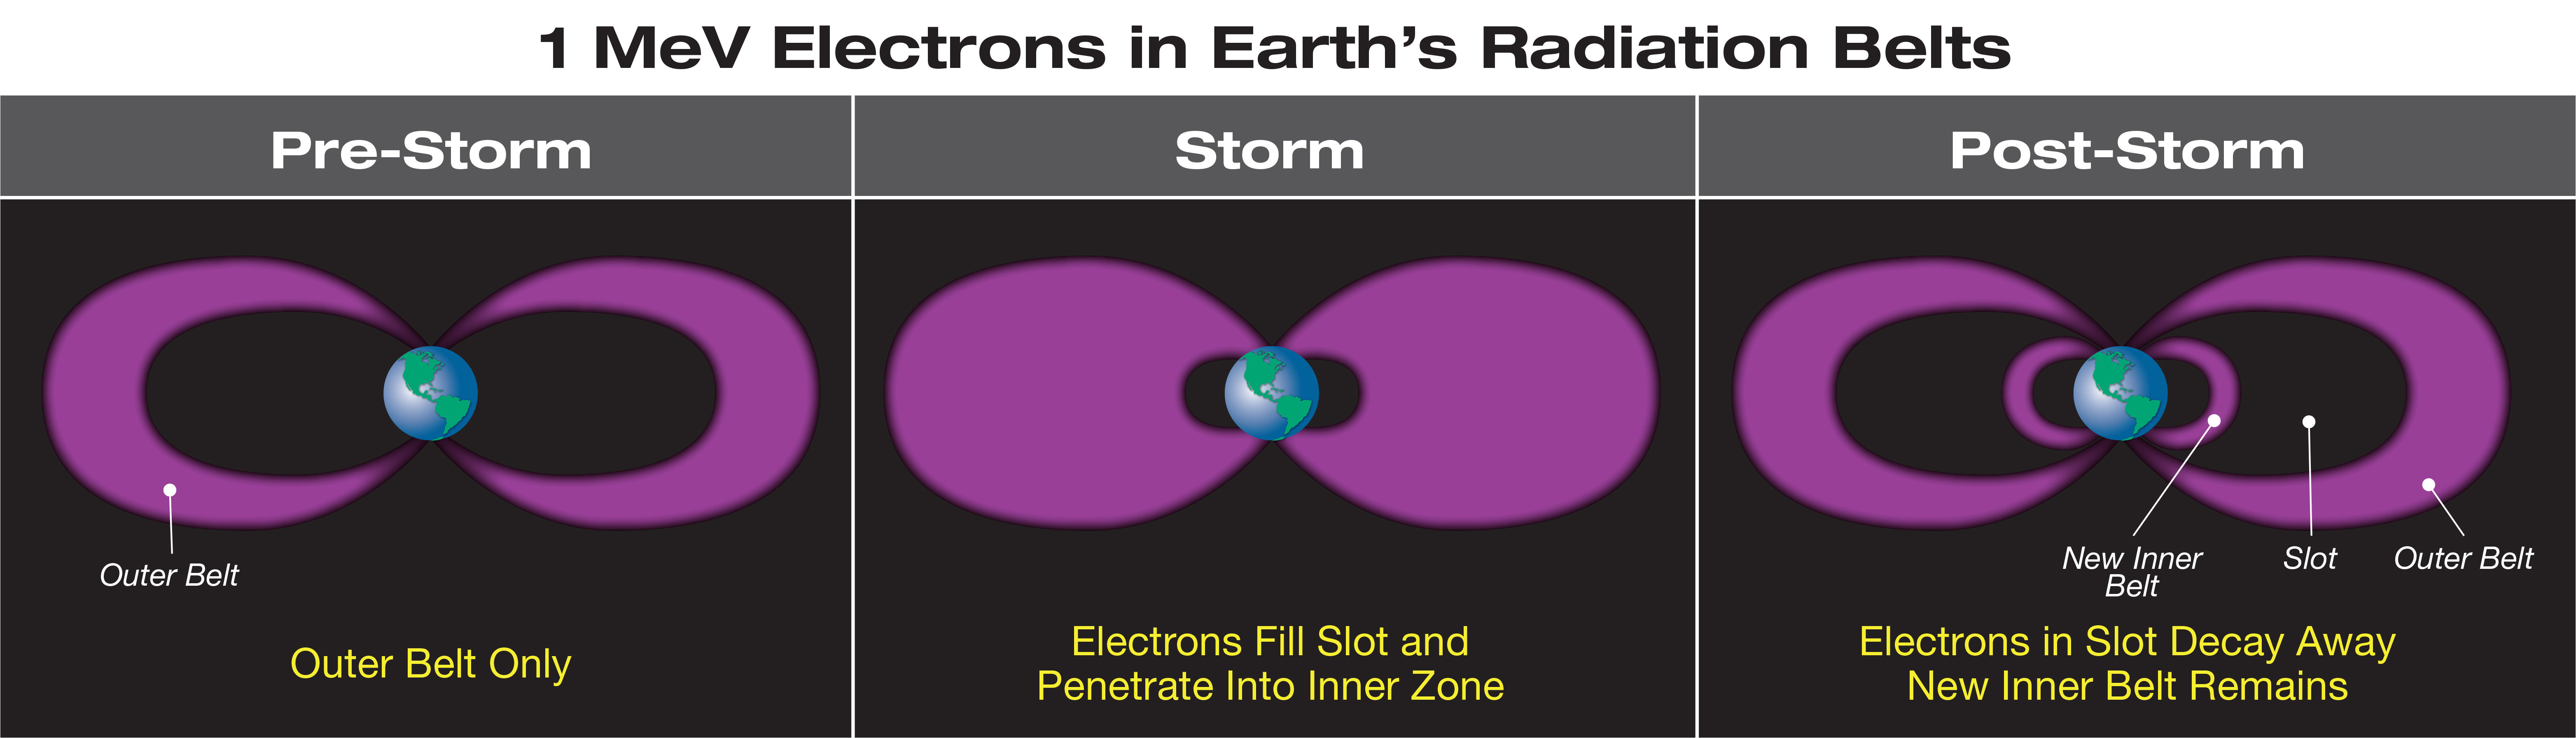
\includegraphics[width=0.7\linewidth]{images/inner_electron_belt_illustration}
	\caption[Образование долгоживущего внутреннего электронного пояса]{ Во время сильных геомагнитный штормов возможно проникновение энергичных электронов во внутренний радиационный пояс. По материалам: NASA’s Goddard Space Flight Center/Mary Pat Hrybyk-Keith \cite{Johnson-Groh2017}}
	\label{fig:innerelectronbeltillustration}
\end{figure}
%\newpage
%===============================================================================

\section{Методы регистрации дозы ионизирующих излучений} \label{sect1_2}

Среди методов регистрации ионизирующих излучений можно выделить несколько наиболее используемых, это газовые ионизационные детекторы, в том числе пропорциональные и газоразрядные счетчики, сцинтилляционные детекторы, полупроводниковые детекторы, трековые детекторы. Наибольшее распространение среди мониторинговых приборов на космических аппаратах получили спектрометры заряженных частиц, так как они позволяют исследовать особенности распространения частиц различных энергий в околоземном пространстве и строить на основе этих данных физические модели радиационных поясов Земли.

Первые эксперименты в космосе по измерению радиационных условий предполагали использование ионизационных камер достаточно большого размера (десятки см\textsuperscript{3}) к этим приборам относятся Р-16 \cite{Mitricas2002} и ионизационные камеры работавшие на шаттлах \cite{Dorman2004}. Современные детекторы радиации в основном строятся на основе полупроводниковых детекторов, хотя ионизационные камеры являются удобным референсным методом, который позволяет провести непрерывный временной ряд исследований вплоть до исследований на первых ИСЗ.

%\newpage
%===============================================================================

\section{Приборы для радиационного мониторинга в космосе} \label{sect1_3}

Дозиметрические и радиационные исследования в космосе не теряют актуальности на протяжении полувека космической эры человечества, это подтверждают актуальные  конференции WRMISS, COSPAR. Большая часть дозиметрических измерений в космосе происходит на космических станциях и в частности на МКС. 
В первую очередь детекторы радиации разделяются на пассивные и активные, хотя такое разделени условно, так как некоторые термо-люминисцентные детекторы и баббл-детекторы можно отнести к активным - они позволяют проводить быстрое считывание данных о дозах на борту космического аппарата. 
%\newpage
%===============================================================================

\subsection{Пассивные детекторы} \label{subsect1_3_1}

Получение информации с пассивных детекторов происходит после накопления порции измерений и требует прерывания цикла измерения. По принципу регистрации излучения они подразделяются на трековые детекторы, термолюминисцентные \cite{Luszik-Bhadra1999,Kulkarni2011} и эмульсионные. 

Детекторы на основе трекового детектора из  тканеэквивалентного пластика CR-39 имеют малый вес, малый объем, лишены электроники, легко обрабатываются и очень дешевы в сравнении с любыми активными дозиметрами \cite{Zhou2008}. 
Пороговое значение LET для материала составляет \~ 5кэВ/мкм. по воде.
Когда заряженные частицы проходят через детектор CR-39,
они теряют энергию за счет ионизации и разрушают молекулярные связи полимера CR-39 с образованием высоко реактивных связей вдоль своих траекторий. Эти траектории могут быть обнаружены в виде вытравленных конусов на поверхностях детекторов CR-39 химическим травлением, эти конусы можно наблюдать с помощью микроскопа. Детекторы CR-39 чувствительны к высоким значениям LET,
могут измерять спектр ЛПЭ, дифференциальный и интегральный флюенс, поглощенную  и эквивалентную дозу для заряженных частиц с высоким ЛПЭ \cite{Zhou2008}. CR-39 может также измерять потоки протонов и нейтронов с высокой энергией через их вторичные заряженные частицы --- осколки столкновений с малым пробегом и высоким ЛПЭ \cite{Zhou2008}. 
Аналогично трековым детекторам на борту МКС применяются также и термолюминисцентные детекторы например: TLD-100, -600, -700, OSLD  \cite{Zhou2010}. Кроме того на БОРТУ МКС проводился эксперимент с системой темолюминисцентных датчиков Pille \cite{Apathy2007}, который был оснащен считывающей системой и позволял относительно оперативно получать данные о дозах в различных позициях в модуле Звезда.

%\newpage
%===============================================================================
\subsection{Активные детекторы} \label{subsect1_3_2}

Для радиационного мониторинга в космическом пространстве используются счетчики частиц, спектрометры и дозиметры. Следует отметить что первые схемы такого рода устройств были предложены еще на заре космических исследований \cite{Markelov1982,Markelov1978} и на данный момент являются незаменимым средством любой космической миссии с участием человека.

К числу полупроводниковых дозиметров относятся приборы ДБ-8, DOSTEL, LIULIN, REM/MPT. Все эти приборы используют принцип регистрации поглощенной дозы в полупроводнике – кремнии, толщиной 300 мкм.  

\subsubsection{ДБ-8}

Дозиметр Бортовой (ДБ) \ref{fig:db} является развитием ряда дозиметрических инструментов применявшихся на различных космических аппаратах для исследовательских целей и штатной работы. ДБ предназначен для регистрации временных вариаций мощности поглощенной дозы и плотности потока частиц СКЛ, ГКЛ, РПЗ. ДБ является детектирующими блоками Системы контроля радиационной (СРК) обстановки ПТК и МКС.

В СРК для МКС используется четыре блока ДБ, что позволяет получить информацию о неоднородности радиационного поля в различных отсеках МКС. 

Регистрируемые данные:
\begin{itemize}
	\item 
	Поглощенная доза в диапазоне - от~10\textsuperscript{-5}~Гр  до~10\textsuperscript{+1}~Гр;  
	\item  
	Мощность поглощенной дозы в диапазоне - от $10^{-10}$~Гр/с  до~$5\cdot10^{-5}$~Гр/с;
	\item  
	Плотность потока частиц в диапазоне от~1 до~$ 10^3 $~частиц/(см$^2\cdot$ с);    		
\end{itemize}



\begin{figure}
\centering
\includegraphics[width=0.7\linewidth]{images/db}
\caption{Внешний вид ДБ --- основных детекторных модулей системы радиационного контроля СРК}
\label{fig:db}
\end{figure}

Прибор содержит 2 узла детектирования, вычислительный блок, блок управления и блок вторичного питания. Оба полупроводниковых детектора в узлах детектирования расположены  параллельно,  образуя телескоп, такая схема построения прибора была использована для получения информации о ЛПЭ частиц, прошедших одновременно через оба детектора.         


Обмен информацией c ДБ обеспечивается по интерфейсу RS-422. Объем целевой информации 2 Мбайта в сутки. Питание ДБ осуществляется постоянным током c напряжением $ 27^{+7}_{-4} $ В. 

\begin{itemize}
\item Энергопотребление ДБ не более 2 Вт.
\item Масса блока 0,25 кг.
\item Габариты ДБ 85×40×100 мм. 
\item Ресурс ДБ  60000 ч, срок службы 12 лет.
\end{itemize}


Поглощенная доза регистрируется узлами с полупроводниковыми детекторами. Для получения информации о величине поглощенной дозы используется принцип регистрации величины заряда в объеме полупроводника, пропорционального энерговыделению в данном объеме. Методы преобразования сигналов с детекторов в цифровую форму и последующая обработка их на микроконтроллере остаются аналогичными алгоритмам, использованным в приборах ДБ-8, ДБ-8М, ДЭПРОН.  


\subsubsection{Liulin}

Детекторы серии Liulin используются с 1988 года, когда их первое поколение было использовано на борту космической станции МИР \cite{Caffrey2011}. Liulin-4 не последний прибор в этой серии, но его простое устройство и компактные размеры обеспечивают удобство использования для многих конкретных задач. Этот спектрометр состоит из единственного кремниевого детектора, зарадочувствительного предусилителя, микроконтроллера и флэш-памяти. Насыщенный литием кремниевый детектор имеет толщину 0,3 мм и площадь 2 см\textsuperscript{2}. В приборе установлен 12-ти битный АЦП, но только 8 бит из них используется для получения 256 канального спектра энерговыделения за выбранный интервал времени накопления: от 10 до 3539 с. Амплитуда импульса определяется после предусилителя и разделяется по 256 энергетическим каналам, начинающимся с 0,02 МэВ до 20 МэВ. Выделение энергии, большее 20 МэВ записывается в наибольший энергетический канал \cite{Dachev2002} .


Для определения дозы в данном типе детектора энерговыделение в каждом канале определяется умножением счета в детекторе на энергию канала. Эти результаты делятся на массу объема детектора и суммируются для определения общей дозы по всем каналам \cite{Dachev2002} \cite{Luszik-Bhadra2010}. Записанная форма спектра энерговыделения может предоставить дополнительную информацию относительно природы доминирующего радиационного поля (ЮАА, ГКЛ и др. ), но не является достаточно подробной для определения ЛПЭ воздействующей радиации \cite{Caffrey2011}. 



Размер и портативность спектрометра типа Liulin-4 делает его жизнеспособным кандидатом для активной персональной дозиметрии во время солнечного события, но ограничения в возможности определения эффективной ЛПЭ и эквивалентной дозы предотвращают вытеснение методов пассивной дозиметрии. Liulin-4 существует во многих модификациях и с многими опциями и может работать как на химическом источнике тока, так и на непрерывном питании, функционировать как с внешним ЖК-дисплеем так и без него, и может включать GPS-приемник \cite{Dachev2002}.	

Впоследствии был разработан также Liulin-5 основным отличие которого является телескоп из трех полупроводниковых детекторов.

В данный момент приборы типа Лиулин используются на нескольких миссиях дальнего космоса как основные дозиметрические устройства \cite{Dachev2015}. Прибор Liulin-MO на ExoMars состоит уже из 4 полупроводниковых детекторов, образующих  боковые грани параллелепипеда \cite{Semkova2015}. Близкий по построению эксперимент Liulin-ML будет отправлен на поверхность Марса в составе активного детектора нейтронов и гамма-излучения (ADRON).

\subsubsection{DOSTEL}

DOSTEL -- Дозиметрический полупроводниковый телескоп был разработан в 1995 году как малый телескоп частиц для использования на миссиях космических шаттлов к космической станции МИР. Прибор включает в себя два кремниевых детектора по технологии PIPS, расположенных как телескоп \cite{Beaujean2002}. Каждый детектор имеет толщину 0,315 мм с чувствительной зоной 6,93 см2, зазор в 15 мм между детекторами дает геометрический фактор 824 см\textsuperscript{2}ср (единица измерения определяется чувствительной площадью детектора и полем зрения) для детектирования совпадающих событий \cite{Beaujean2002}. Каждый детектор соединен с зарядочувствительным усилителем через интегрирующую емкость, двух стадийным усилителем импульсов, двумя пиковыми детекторами, двумя RC-фильтрами для снижения уровня шумов и 8-ми битным АЦП. Такая компоновка позволяет поводить анализ амплитуд импульсов отдельно для высокого и низкого энергетического диапазона \cite{Beaujean2002}.


Когда совпадающее событие записано обоими детекторами, становится возможным определить ЛПЭ падающего излучения. Так как известно, что траектория частицы ограничена конусом возможных направлений, средняя толщина детектора может быть использована для оценки длины трека частицы. Делением энерговыделения на среднюю длину свободного пробега, для данного детектора 0,364 мм \cite{Beaujean2002} с плотностью 2,33 г/см\textsuperscript{3}  можно получить приближенное значение ЛПЭ \cite{knoll2000radiation}. Результат таких вычислений нормируется на известный коэффициент для перехода от ЛПЭ кремнии к ЛПЭ в воде, таким образом прибор DOSTEL записывает ЛПЭ в диапазоне от 0,1 до 240 кэВ/мкм \cite{Beaujean2002}.


\subsubsection{REM/MPT}
\begin{figure}
	\centering
	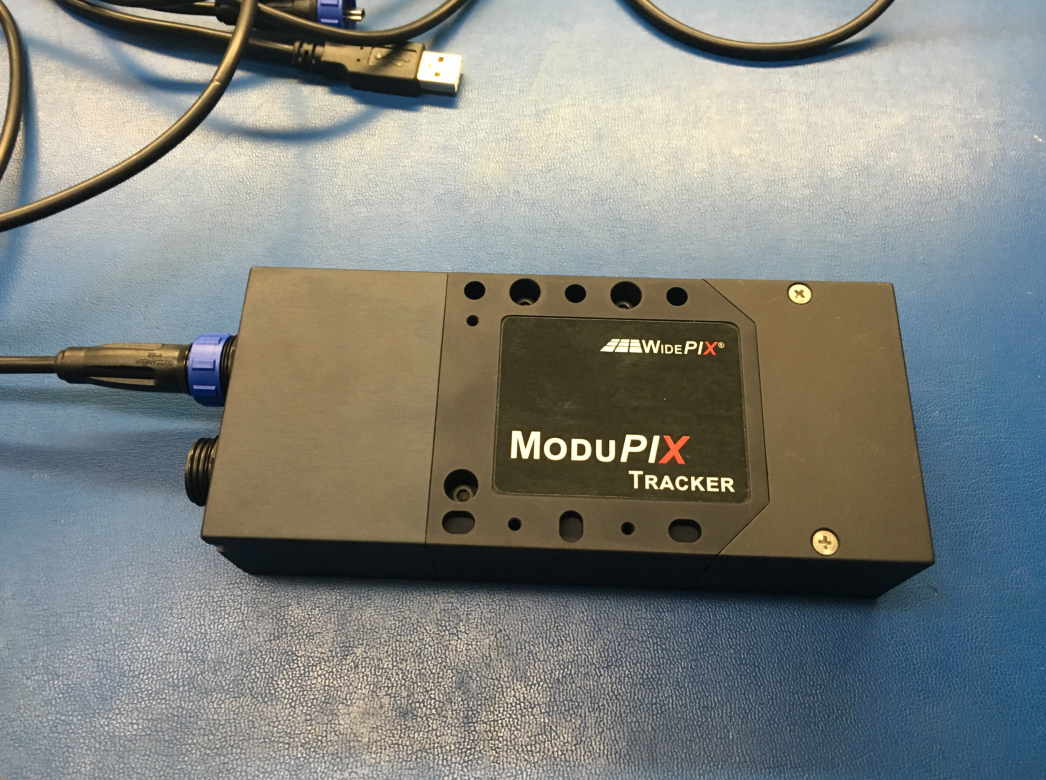
\includegraphics[width=0.49\linewidth]{images/remmodupix}
	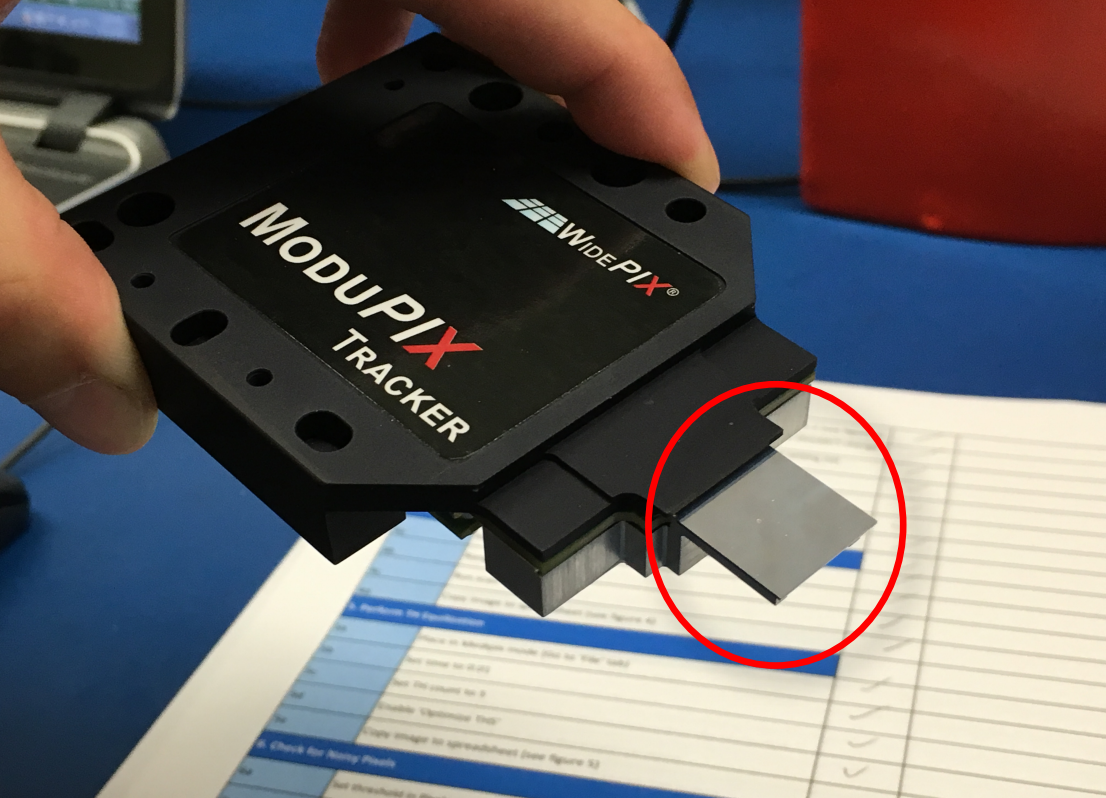
\includegraphics[width=0.49\linewidth]{images/modupix}
	\caption{Один из модулей ModuPIX прибора REM}
	\label{fig:modupix}
\end{figure}



Существенным отличием установленного NASA на МКС прибора Radiation Environment Monitor (REM) от других полупроводниковых дозиметров  является позиционно-чувствительная система считывания энерговыделений в детекторе. Эта особенность при телескопическом расположении детекторов позволяет производить значительно более точные оценки энерговыделения каждой частицы с помощью дополнительной информации о угле падения частиц. Каждый детектор представляет собой матрицу 256 X 256 пикселей размером 14х14 мм, и считывается со скоростью до 850 кадров/с.

Прибор REM включает сенсорные платы Medipix 3-го поколения. Medipix 1, 2 и 3го поколения это серия пикселизованных детекторов фотонов и заряженных частиц разрабатываемых с 1990-х годов большой коллаборацией институтов под эгидой CERN. На основе данных микросхем были построены приборы регистрации радиации для МКС с 2013 года и для первых тестов многоцелевого аппарата Орион в 2014 году.

Обработка сигнала с каждого пикселя производится поэлементно и реализована на Asic микросхеме ридаут Timepix. На данный момент известно, что исследования на борту МКС продолжатся в марте 2017 году, а разработкой новой аппаратуры занимается Европейская компания Advacam, производящая микросхемы Medipix. Для этой цели разрабатывается прибор Miniaturized Particle Telescope (MPT)\cite{Fry2016} - представляет собой телескоп из двух детекторов построенный на основе Timepix технологии \cite{Kroupa2015}, и по сути представляет собой два прибора REM. 

Для миссии на МКС прибор оснащен двумя USB коннекторами и подключается к ноутбуку, данные считываются ежедневно а обработка данных будет производится на Земле. В перспективе данный прибор рассматривается как основное дозиметрическое средство на борту КА Орион, полеты которого запланированы с сентября 2018 года.


\subsubsection{ELFIN}
Прибор ELFIN входит в состав аппаратуры КА Ломоносов и является спектрометром в отличии от других описанных приборов. Прибор состоит из двух полупроводниковых телескопов с алюминиевой и танталовой защитой, которая по мнению изготовителей будет необходима для работы в радиационных поясах.\cite{VassilisAngelopoulos}

\begin{figure}
	\centering
	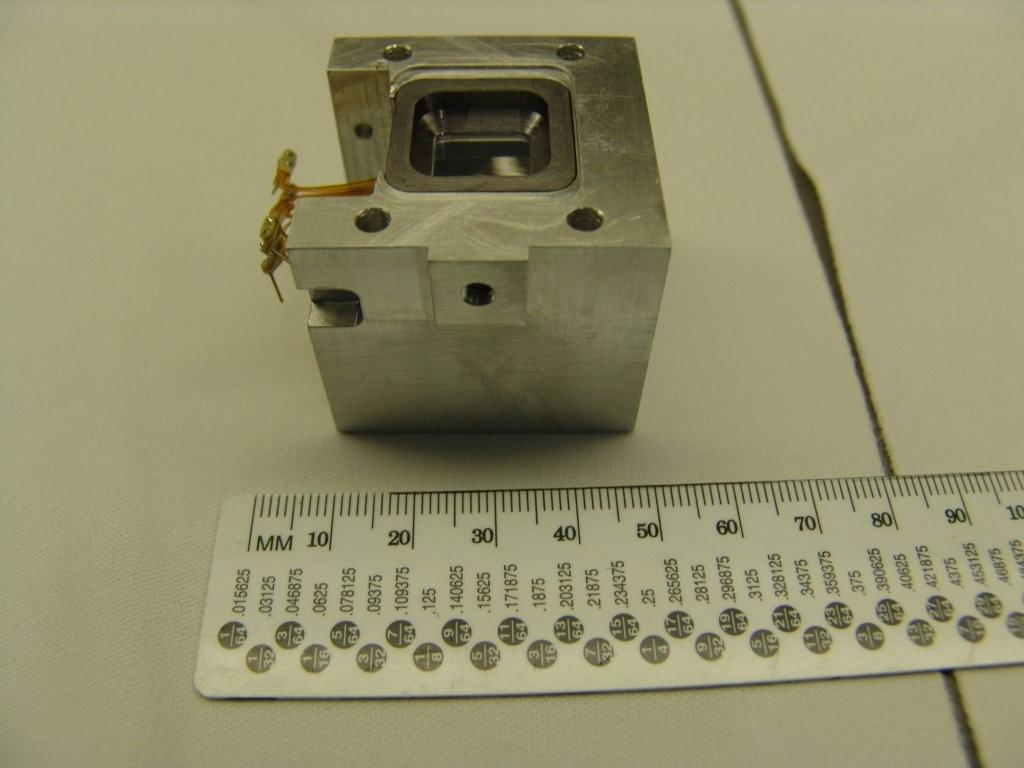
\includegraphics[width=0.33\linewidth]{images/elfin/DSC04260}
	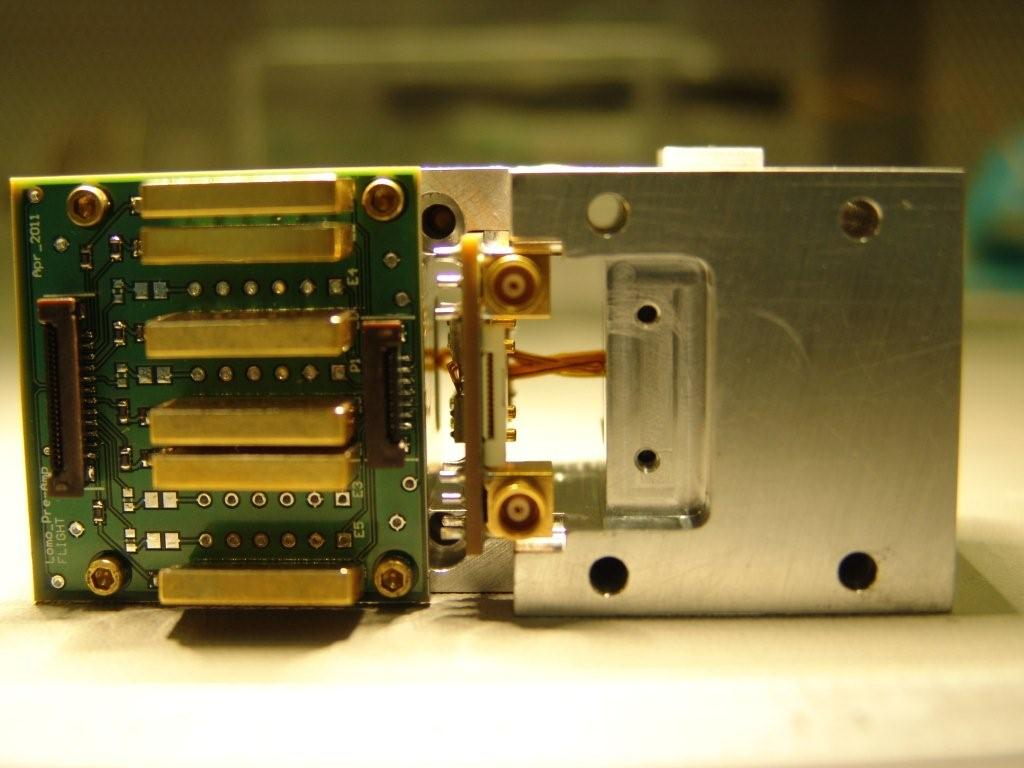
\includegraphics[width=0.33\linewidth]{images/elfin/DSC04287}
	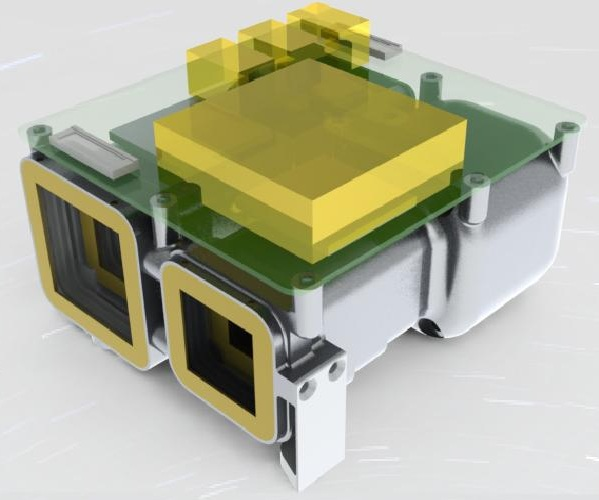
\includegraphics[width=0.32\linewidth]{images/EPD_Brochure}
	\caption{Устройство телескопа детекторов для электронов с входным окном (слева). 	Плата предусилителей со сборкой плат электроники (в центре). Модель прибора ELFIN (справа) }
	\label{fig:dsc04260}
\end{figure}


Параметры прибора :
\begin{itemize}
	\item Диапазон измерения электронов: 50 кэВ до 4 МэВ
	
	\item Диапазон измерения ионов: 50 кэВ до 500 кэВ
	
	\item Геометрические факторы:
	
	\begin{itemize}
		\item Электроны: 0.04см$ ^{2}\cdot $ср
		
		\item Ионы: 0.003см$ ^{2}\cdot $ср
	\end{itemize}
	
	
	\item dE/E < 50\%
	
	\item Масса прибора менее 1.5 кг включая защиту детектора 1.2 см из Al+Ta
	
	\item Габариты 85 x 80 x 80 mm
\end{itemize}

В состав прибора входит магнитометр, необходимый для выяснения связи локальных магнитных условий в месте нахождения спутника и потоков электронов, покидающих радиационные пояса. С целью выявления популяции высыпающихся частиц ось телескопов прибора направлена примерно в конус потерь - на 60 линейных градусов от зенита.







\subsubsection{MSL/RAD}
Прибор Radition Assesment Detector (RAD) предназначен для оценки радиационных условий на Марсианской лаборатории Curiosity. Он состоит из детектора заряженный и нейтральных частиц\cite{Zeitlin2016}. Этот первый прибор для измерения спектра частиц и мощности дозы на пути к марсу и на его поверхности \cite{Matthia}.

RAD позволяет раздельно регистрировать потоки заряженных и нейтральных частиц, так как прибор предназначен для измерения дозы на поверхности Марса, где значительный вклад в дозу вносят нейтроны и гамма кванты, образованные при взаимодействии ГКЛ с марсианской почвой \cite{Zeitlin2010}. В процессе разработки прибора прошел градуировку и калибровку на двух ускорителях ионов (протонов, углерода, гелия, железа), нескольких источниках ИИ и 4 источниках нейтронов и гамма-лучей энергиями от 5  до 100 МэВ \cite{Zeitlin2010}. Данные полученные на источниках излучений прошли сравнение с данными, полученными с помощью моделирования Монте-Карло.


\begin{figure}
	\centering
	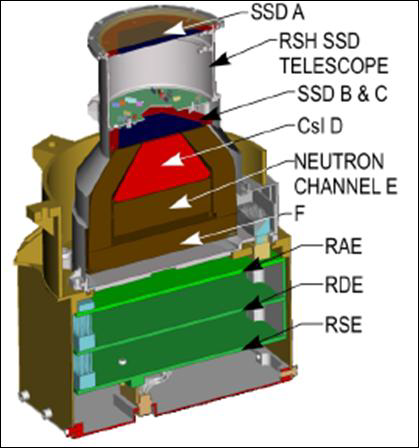
\includegraphics[width=0.33\linewidth]{images/radmsl1}
	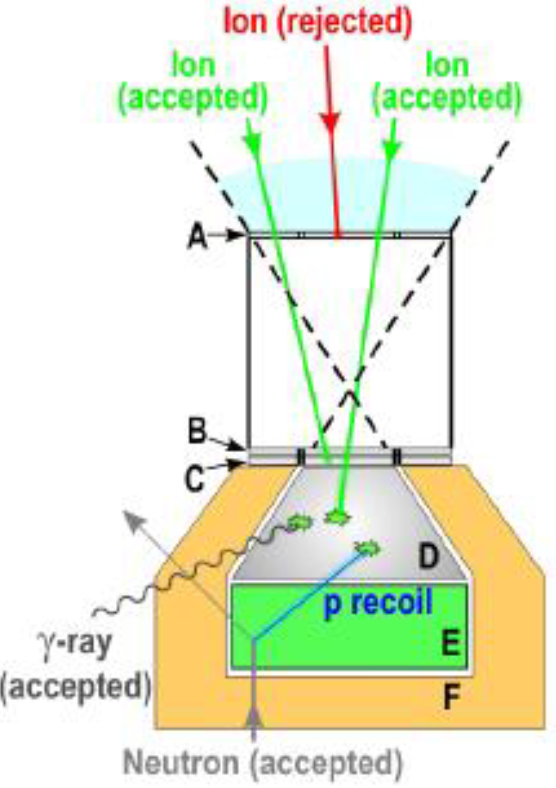
\includegraphics[width=0.30\linewidth]{images/radmsl}
	\caption[Внутреннее устройство прибора RAD.]{Внутреннее устройство прибора RAD. Входное окно образовано 300 мкм полупроводниковыми детекторами A, B и C для определения ЛПЭ излучения. Нейтральные частицы регистрируются в кристалле CsI(D) и пластиковом сцинтилляторе (E). Сцинтилляторы окружены антисовпадательной защитой(А).}
	\label{fig:radmsl}
\end{figure}

Электроника прибора состоит из четырех предусилителей, данные с которых захватываются и дискриминируются с помощью ASIC модуля VIRENA, единственное АЦП управляется модулем VIRENA и передает оцифрованные данные на FPGA, осуществлявшее цифровую обработку данных, и далее на другую FPGA, для сохранения и передачи данных. 

Прибор RAD показал что доза на поверхности Марса модулируется гелиосферным магнитным полем и коррелирует с атмосферным давлением \cite{Guo2017}. Доза в течении одного сола меняется на 10 процентов, находясь в противофазе с давлением и составляет в среднем 200 мкГр/сутки.




R-16 Pulse-type ion chamber: 1 pulse per 5 mrad; shallow and deep dose rates; assumes average LET [Mitricas et al. (2002), Badhwar (2000)]


BBND Heavy system; short-term experiment; requires 3He Koshiishi et al. (2007), Matsumoto et al. (2001)

\subsubsection{SEISS}
Группа радиационных приборов SEISS установлена на GOES-R (GOES-16)\cite{Goodman2013}, который запущен 19 ноября 2016 года. 
Пакет приборов Seiss состоит из: детектора тяжелых ионов  (EHIS), детектора частиц РПЗ - высокого и низкого (MPS-HI и MPS-LO) и детектора солнечных и галактических протонов (SGPS). Планируется что данные из Seiss будут использоваться для предупреждений о опасных явлениях космической погоды, а также улучшит прогнозы потоков энергичных частиц. 

\subsubsection{MEPED}
Сеть полярных операционных спутников Земли (POES) полярно-орбитальных космических аппаратов представляет собой комплекс спутников с наиболее близкими орбитами к орбите Ломоносова и поэтому схожими по радиационным условиям полета. Особый интерес для магнитосферных исследований представляет подсистема Space Environmental Monitor, предназначенная для измерения потоков частиц на низкой околоземной орбите, сейчас она представлена ​​в обновленной конфигурации (SEM -2), эта подсистема является содержит приборы среднего протонного и электронного детекторов (MEPED).
В состав MEPED входят в общей сложности восемь приборов в диапазоне от 30 кэВ до 200+ МэВ (для протонов) и от 30 до 2500 кэВ (для электронов).

Интересно, что низковысотные, полярно-орбитальные спутники NOAA POES проявляют побочный отклик на релятивистские электроны в приборе MEPED\cite{Yando2011}.
\begin{figure}
	\centering
	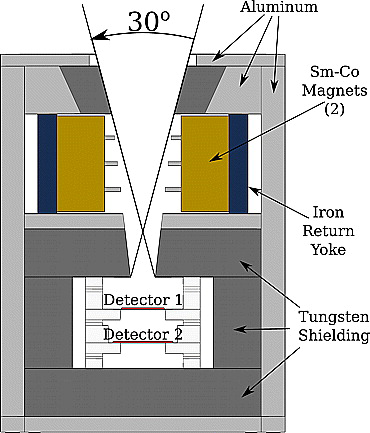
\includegraphics[width=0.3\linewidth]{images/jgra21383-fig-0002}
	\caption{Схема прибора протонного телескопа MEPED, показанного в поперечном разрезе.\cite{Yando2011}}
	\label{fig:jgra21383-fig-0002}
\end{figure}


\subsection{Детекторы нейтронов} \label{subsect1_3_1}


Достоверно известно что нейтроны также вносят ощутимый вклад в эквивалентную дозу и по разным оценкам достигает 20-30\% \cite{Dudkin1990}, а для эффектов обусловленных ядерным взаимодействием (в том числе повреждения ДНК, эффектов пробоя в микроэлектронике и биологической эквивалентой дозе) может достигать 50-60\% \cite{Armstrong2001} \cite{Benton2001}. Кремниевые детекторы имеют низкую чувствительность к нейтронному излучению, поэтому для регистрации ожидаемых в космическом пространстве потоков нейтронов \cite{Esteban2016} и используются детекторы конвертирующие нейтроны в заряженные частицы или газонаполненные счетчики \cite{Stozhkov2007}.Методы регистрации нейтронов с использованием конвертеров были предложены еще в 1959 году \cite{McGregor2013}. Основным недостатком данный методики регистрации является низкая эффективность конвертирования нейтронов --- около 1\% для плоских покрытий и 8\% для более сложных конструкций конвертеров на основе $ ^{10} $B и $ ^6 $LiF детекторов \cite{Mendicino2015}. В последнее время наблюдается серьезный прогресс в создании новых детекторов такого типа и по оценкам эффективность их может достигать 40\% \cite{McGregor2013}. 

На станциях МИР и МКС распространенной техникой регистрации нейтронный полей была дозиметрич на основе термолюминисцентных детекторах. В качестве термолюминисцентных материалов использовались пластиковые сцинтилляторы CR-39 \cite{Alberts1991}, оксид алюминия с добавками $ ^6 $LiF, тефлона и полиэтилена\cite{Kulkarni2011}.

 В НИИЯФ МГУ также разрабатывались приборы для контроля уровня нейтронного излучения \cite{Shavrin1990} и успешно применялись на ряде спутниковых экспериментов. Данные приборы построены на принципе регистрации реакции нейтронов с $ ^{3} $He. Сечение взаимодействия реакции захвата нейтроны гелием велико только для тепловых нейтронов, поэтому для регистрации энергичных нейтронов требуется окружение счетчиков замедлителем \cite{Shavrin2002}.

Особенно интересны радиобиологические исследования проведенные в ИМБП \cite{Shurshakov2016} на МКС с использованием тканеэквивалентного фантома Матрешка, показывающие что вклад нейтронов в дозу может достигать 28\%.  Исследования при этом производились по методике определения количества пузырьков в ``Баббл-дозиметре'' \cite{hulapko2016}.


Известен нейтронный детектор для эксперимента Памела \cite{Menn2013}, он размещен непосредственно под счетчиком S4 с целью увеличения электромагнитной и адронной способности распознавания прибора Памела и расширения энергетического диапазона первичных протонов и электронов до $ 10^{11}-10^{13} $ эВ. Детектор состоит из 36 счетчиков  $ ^{3} $He, упакованных в полиэтиленовый замедлитель толщиной до 9 см, способных детектировать тепловые нейтроны с эффективностью 10\%, учитывая эффективность термализации нейтронов, образующихся в калориметре.

\begin{figure}
	\centering
	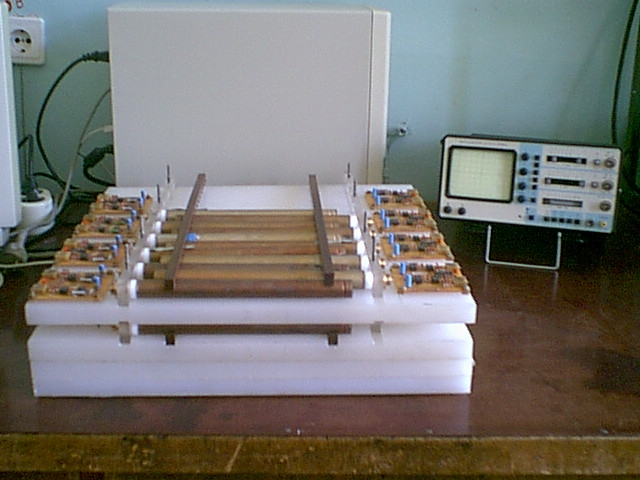
\includegraphics[width=0.7\linewidth]{images/neutrons/pamela}
	\caption{Устройство кассеты нейтронных счетчиков для эксперимента PAMELA \cite{Stozhkov2007}}
	\label{fig:pamela}
\end{figure}

Размер нейтронного детектора составляет 60x55x15 см$ ^3 $, общий вес - 30 кг, потребляемая мощность - 10 Вт. Регистрируется всенаправленный поток частиц, за исключением углов, экранированных магнитом PAMELA, защитой из пластин Cd и Землей, а геометрический фактор достигает 900 см$ ^2 $ ср \cite{Stozhkov2007}. Авторами детектора производились попытки для анализа нейтронных потоков от Солнца, однако однозначного результата получить не удалось \cite{Goryacheva2016}. Результаты анализа совпадений триггеров спектрометра и колориметра эксперимента с триггерами нейтронного детектора дают основания полагать что около 75\% нейтронов образуются в массе космического аппарата \cite{Stozhkov2007}.

Также известно что счетчики нейтронов используются на орбите Марса и позволили получить важный научный результат о наличии воды на поверхности Марса.  Этот  результат получен с помощью прибора HEND \cite{Feldman2004}. Аналогичные приборы для обнаружения воды с помощью регистрации потока нейтронов разработаны для работы на поверхности (DAN \cite{Mitrofanov2012a}) и орбите марса. На аппарате ExoMars2016 установлен FREND \cite{Mitrofanov2012}. С помощью четырех гелиевых счетчиков прибор позволит регистрировать околотепловые нейтроны 0.4–500 кэВ и заряженные частицы 0.5–10 MeV, с помощью сцинтилляционного детектора. Сужение поля зрения прибора произведено двухслойным коллиматором, внешний слой из полиэтилена замедляет нейтроны, а внутренний из $ ^10 $B поглощает их. 

Интересно что данный прибор работает в паре с дозиметрическим модулем Liulin-MO и таким образом композиция этих двух приборов представляет собой очень близкий аналог прибора ДЭПРОН.
\begin{figure}
	\centering
	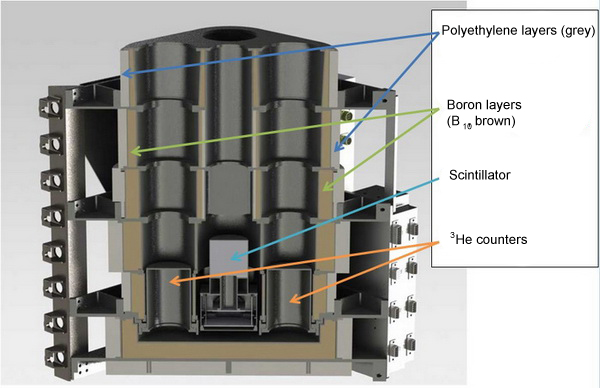
\includegraphics[width=0.7\linewidth]{images/frend3-eng}
	\caption{Устройство прибора FREND \cite{Mitrofanov2012}}
	\label{fig:frend3-eng}
\end{figure}

%\newpage
%===============================================================================
\section{Математическое моделирование дозиметрических приборов для космических условий}

Математическое моделирование широко применяется на всех этапах создания исследовательских проборов предназначенных для использования в условиях космоса. В первую очередь оно необходимо на этапе проектирования аппаратуры для выбора характеристик регистрирующих радиацию модулей исходя из поставленных экспериментальных задач \cite{Hassler2008}. На последующих шагах разработки аппаратуры математические методы используются при верификации результатов калибровочных и градуировочных испытаний на источниках ИИ и ускорителях заряженных частиц \cite{Zeitlin2010, Luszik-Bhadra2008} . Также одним из основных применений является уточнение функции отклика прибора во время штатной работы \cite{Zeitlin2010}. 


Среди математических методов моделирования взаимодействия ИИ и нейтральных излечений с материалами и детектирующими модулями приборов следует отметить наиболее используемые программные пакеты, основанные на методе Монте-Карло:


\begin{description}
	\item[GEANT4] комплекс программ для моделирования прохождения частиц через вещество\cite{Allison2006},  код общедоступен;
	\item[SHIELDOSE ] система расчетов доз за секционированной защитой \cite{SeltzerS.M.1980},  код общедоступен;
	\item[PHITS] Система расчета перемещений частиц и тяжелых ионов, 
	разработана в Японии и Австрии \cite{Niita2006, Sato2006} ;
	\item[HZETRN] код использующийся NASA для расчетов радиационных условий в космосе \cite{Heinbockel2009},  код общедоступен;
	\item[FLUKA] система широко использующаяся в CERN для широко круга задач и 
	первую очередь для медицинских приложений\cite{Fasso2003, fluka2014}.
\end{description}

Далее рассмотрен только пакет Geant4, так как в настоящей работе именно этот пакет 
был выбран для расчетов. 


\subsection{GEANT4}

Данная система математического моделирования разрабатывается для нужд работы 
ЦЕРН и активно используется в ряде областей науки, медицины и технологии 
\cite{Agostinelli2003}.
К настоящему моменту система Geant4 развилась настолько, что от основной ветки 
разработки отделилось несколько специализированных продуктов, использующих 
только ядро системы для расчетов распространения частиц. Основные направления 
развития это микродозиметрические исследования(GEMAT), применение к 
распространению и 
воздействия космического излучения(GRAS, PLANETOCOSMICS ), оптимизация 
экранирования (MULASSIS \cite{Lei2002} и SSAT). 

Следует отметить что многие из упомянутых программ организованы в единый комплекс Spenvis,
 из них особенно применим для исследований характеристик приборов  Geant4 Radiation Analysis for Space (GRAS) \cite{Santin2005}. Этот пакет принимает в качестве входных данных GDML файл с моделью прибора и позволяет автоматически создавать комплексные источники космического излучения соответствующие различным орбитам полета спутников.

%\newpage
%===============================================================================
\section{Возможности КА Ломоносов в продолжении ряда российских исследований радиационной обстановки}

На многих российских пилотируемых кораблях со времен первого полета человека в космос устанавливались дозиметрические приборы, изготовленные в НИИЯФ МГУ, исчерпывающий список и результаты этих экспериментов можно найти в монографии Ю.И. Логачева 2007г \cite{logachev2007}. Отличительной чертой данного эксперимента является возможность прозондировать более высокие широты по сравнению с орбитами таких комплексов как станция МИР и МКС. 

Вторым но не менее важным моментом является уникальное сочетание многих исследовательских приборов на одном аппарате, такое сосредоточение позволяет получить уникальную информацию о множестве параметров исследуемых явлений, будь то гамма вспышки земного или неземного происхождения, или транзиентные явления в верхней атмосфере - такие как эльфы и спрайты. Дозиметрический прибор поможет отследить сбойные явления в аппаратуре КА, связанные с повышением уровня радиации и отделить их от ценных научных данных. А также, дать новую информацию о явлениях в авроральных областях, высыпаниях во внешнем радиационном поясе.

На борту спутника кроме прибора ДЭПРОН установлены два прибора позволяющие регистрировать различные компоненты радиационной нагрузки, это БДРГ --- Блок детектирования рентгеновского и гамма излучения (НИИЯФ МГУ), ELFIN (UCLA и IGPP) --- прибор для обнаружения высыпаний электронов и исследования магнитных полей, содержащий детектор электронов и ионов (EPD-E и EPD-I), наряду с магнитометром. Такая тройка приборов позволяет при небольшом весе проводить разносторонние измерения параметров радиационной обстановки.


%\centering
%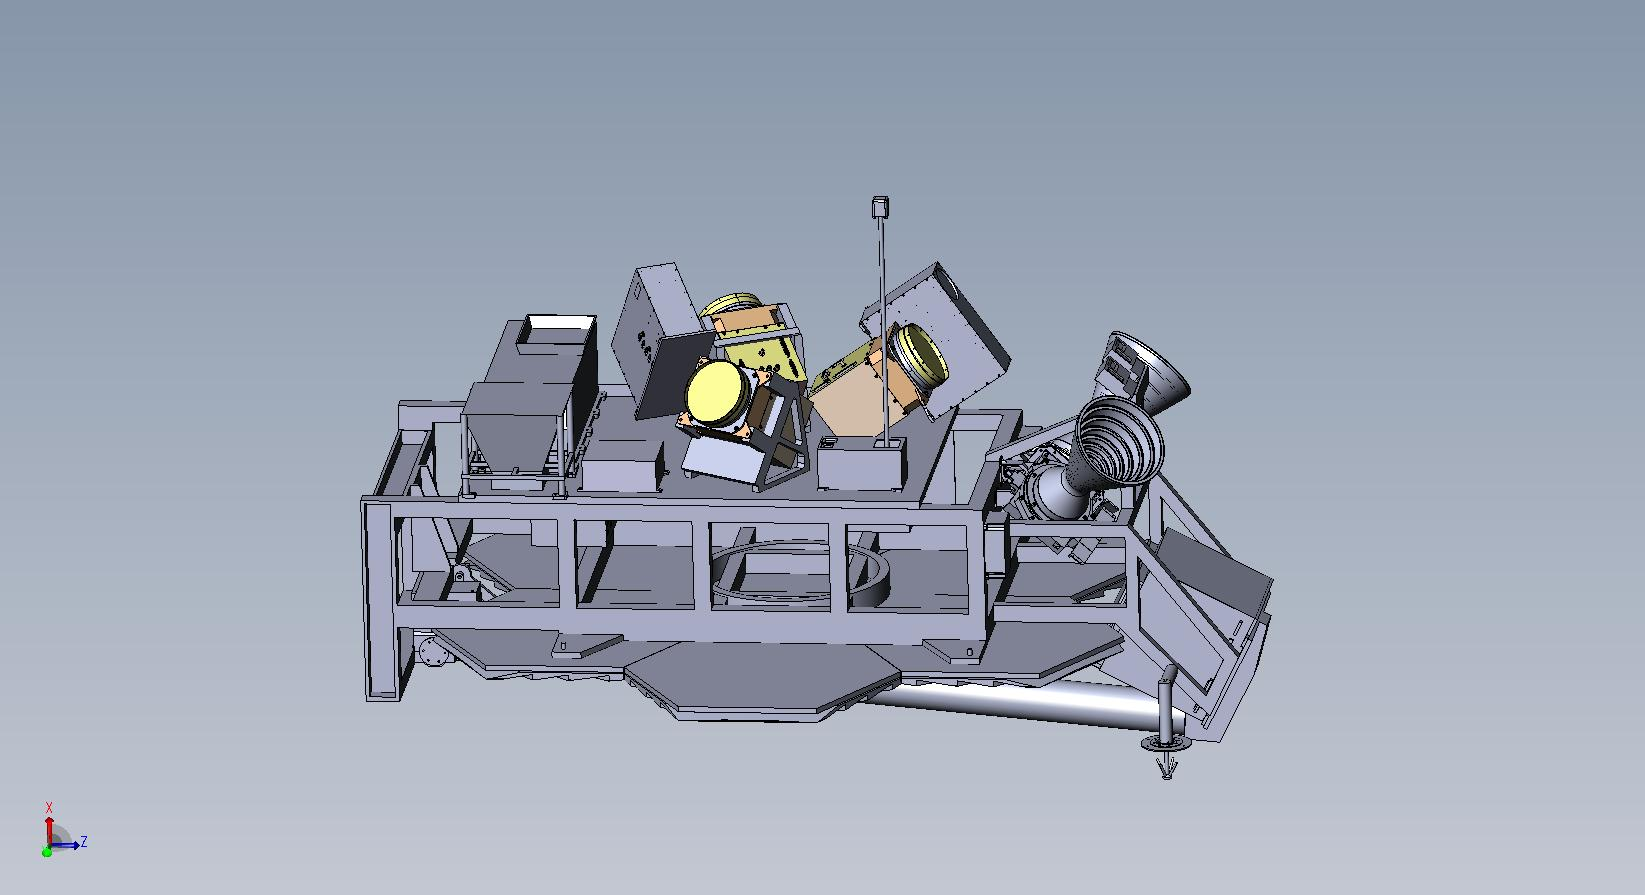
\includegraphics[width=0.8\linewidth]{images/lomonosov2}
%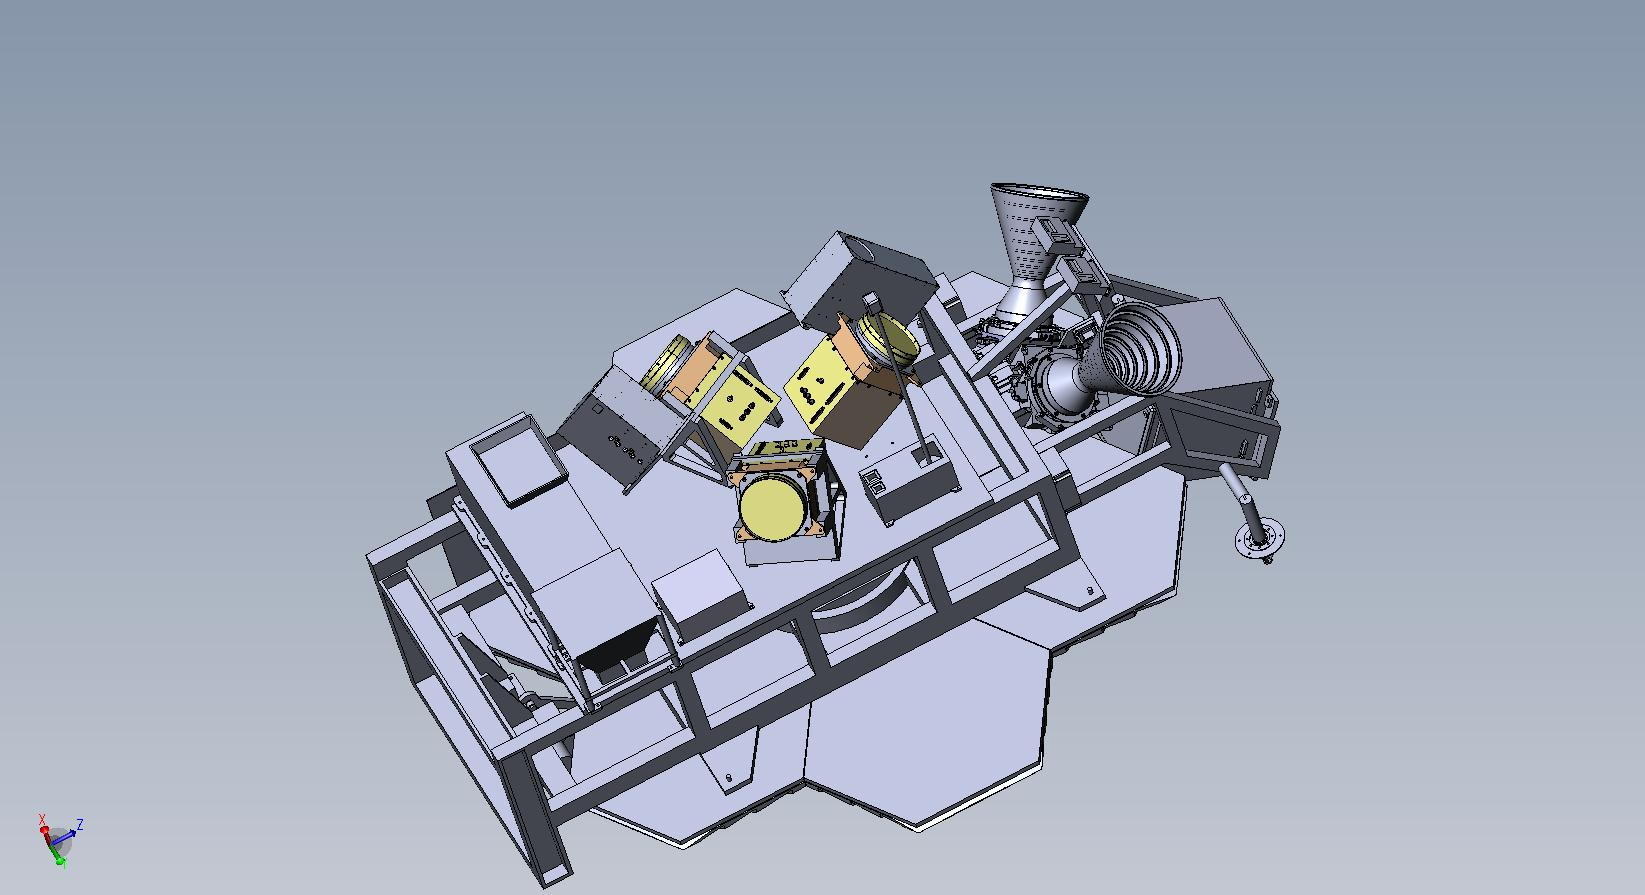
\includegraphics[width=0.8\linewidth]{images/lomonosov1}
%\caption{Внешний вид спутника Ломоносов старый}
%\label{fig:lomonosov2}
%\end{figure}

\begin{figure}
\centering
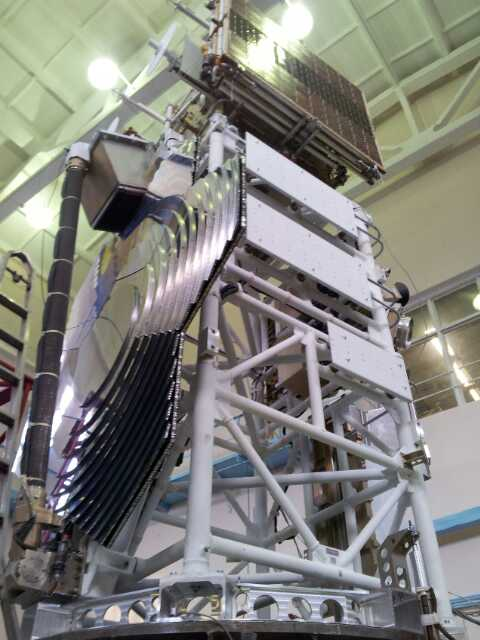
\includegraphics[height=7cm,keepaspectratio]{images/lomo4}
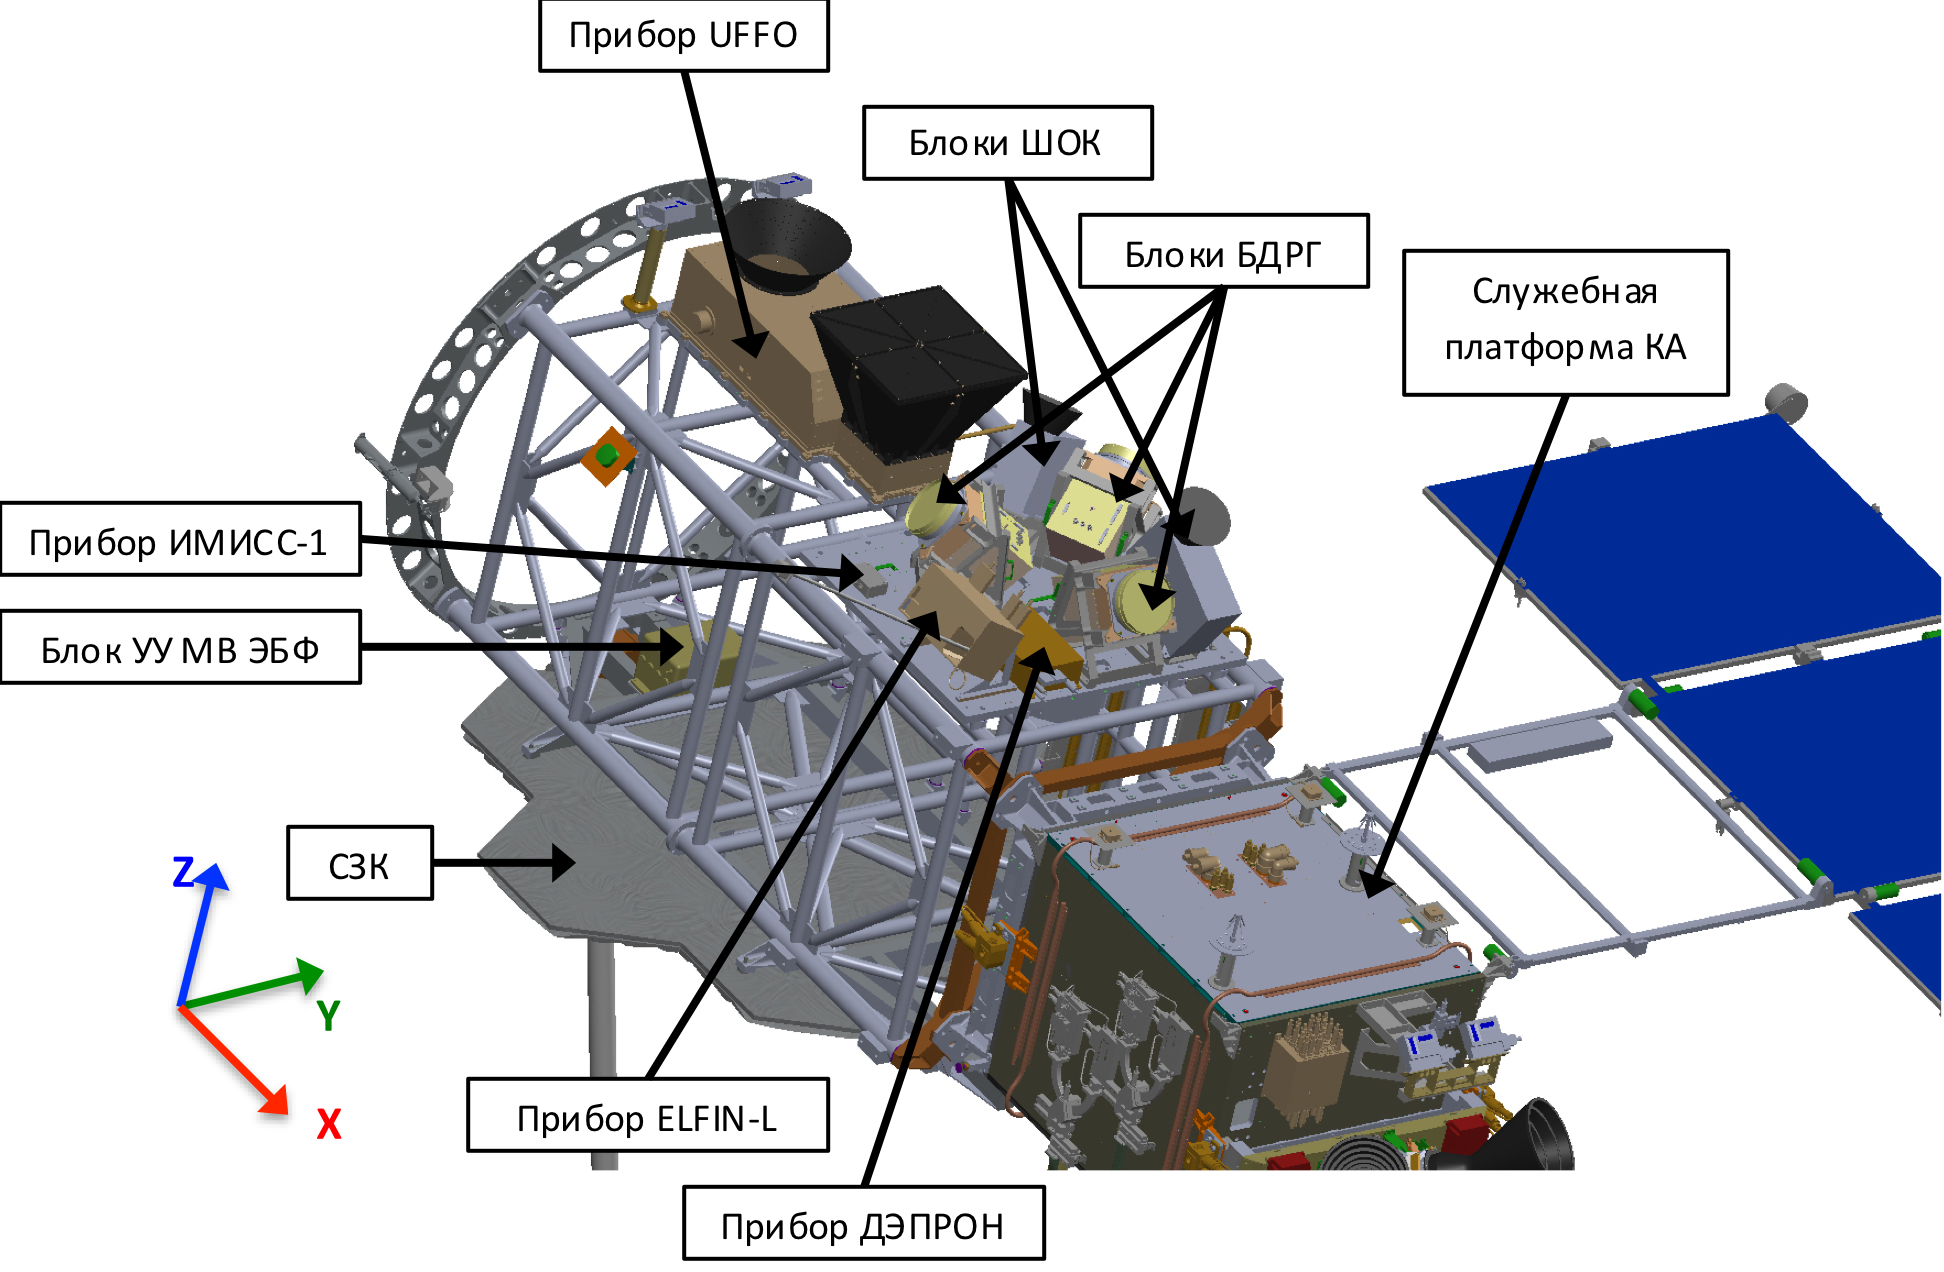
\includegraphics[height=7cm,keepaspectratio]{images/lomo3}
\caption{Внешний вид спутника Ломоносов и относительное расположение приборов}
\label{fig:lomo3}
\end{figure}


